\pgfsetplotmarksize{0pt}
\begin{figure}
 \centering
 \caption{\label{fl_conv5}FLClustered/test5.txt},
 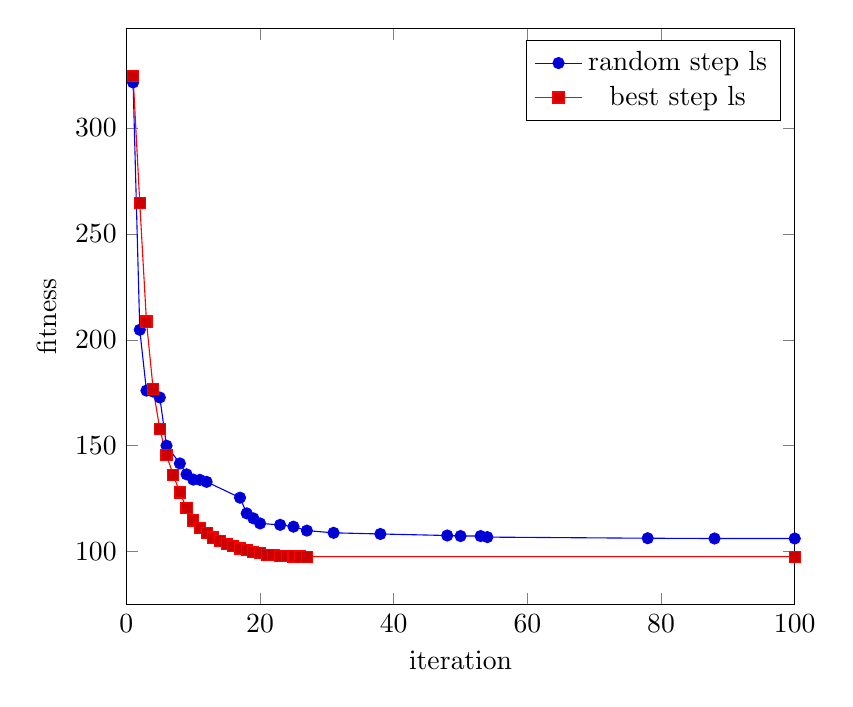
\begin{tikzpicture}
 \begin{axis}[
   width=0.7\textwidth,
   scale only axis,
   xlabel=iteration,
   ylabel=fitness,
   xmin=0,xmax=100,
   domain=0:100]
   \addplot coordinates {
     (0,inf)
     (1,321.516)
     (2,204.71)
     (3,176.002)
     (4,175.545)
     (5,172.737)
     (6,149.988)
     (8,141.604)
     (9,136.452)
     (10,133.981)
     (11,133.856)
     (12,132.915)
     (17,125.433)
     (18,118.026)
     (19,115.677)
     (20,113.278)
     (23,112.6)
     (25,111.752)
     (27,109.885)
     (31,108.84)
     (38,108.297)
     (48,107.575)
     (50,107.329)
     (53,107.316)
     (54,106.817)
     (78,106.287)
     (88,106.156)
     (100,106.156)
   };
   \addlegendentry{random step ls}
   \addplot coordinates {
     (0,inf)
     (1,324.436)
     (2,264.543)
     (3,208.62)
     (4,176.78)
     (5,157.734)
     (6,145.559)
     (7,136.147)
     (8,127.923)
     (9,120.485)
     (10,114.688)
     (11,111.168)
     (12,108.64)
     (13,106.607)
     (14,105.006)
     (15,103.566)
     (16,102.425)
     (17,101.445)
     (18,100.644)
     (19,99.8702)
     (20,99.1586)
     (21,98.5503)
     (22,98.2343)
     (23,97.9319)
     (24,97.7624)
     (25,97.6722)
     (26,97.6188)
     (27,97.5988)
     (100,97.5988)
   };
   \addlegendentry{best step ls}
 \end{axis}
 \end{tikzpicture}
\end{figure}
